
% Default to the notebook output style

    


% Inherit from the specified cell style.




    
\documentclass[11pt]{article}

    
    
    \usepackage[T1]{fontenc}
    % Nicer default font (+ math font) than Computer Modern for most use cases
    \usepackage{mathpazo}

    % Basic figure setup, for now with no caption control since it's done
    % automatically by Pandoc (which extracts ![](path) syntax from Markdown).
    \usepackage{graphicx}
    % We will generate all images so they have a width \maxwidth. This means
    % that they will get their normal width if they fit onto the page, but
    % are scaled down if they would overflow the margins.
    \makeatletter
    \def\maxwidth{\ifdim\Gin@nat@width>\linewidth\linewidth
    \else\Gin@nat@width\fi}
    \makeatother
    \let\Oldincludegraphics\includegraphics
    % Set max figure width to be 80% of text width, for now hardcoded.
    \renewcommand{\includegraphics}[1]{\Oldincludegraphics[width=.8\maxwidth]{#1}}
    % Ensure that by default, figures have no caption (until we provide a
    % proper Figure object with a Caption API and a way to capture that
    % in the conversion process - todo).
    \usepackage{caption}
    \DeclareCaptionLabelFormat{nolabel}{}
    \captionsetup{labelformat=nolabel}

    \usepackage{adjustbox} % Used to constrain images to a maximum size 
    \usepackage{xcolor} % Allow colors to be defined
    \usepackage{enumerate} % Needed for markdown enumerations to work
    \usepackage{geometry} % Used to adjust the document margins
    \usepackage{amsmath} % Equations
    \usepackage{amssymb} % Equations
    \usepackage{textcomp} % defines textquotesingle
    % Hack from http://tex.stackexchange.com/a/47451/13684:
    \AtBeginDocument{%
        \def\PYZsq{\textquotesingle}% Upright quotes in Pygmentized code
    }
    \usepackage{upquote} % Upright quotes for verbatim code
    \usepackage{eurosym} % defines \euro
    \usepackage[mathletters]{ucs} % Extended unicode (utf-8) support
    \usepackage[utf8x]{inputenc} % Allow utf-8 characters in the tex document
    \usepackage{fancyvrb} % verbatim replacement that allows latex
    \usepackage{grffile} % extends the file name processing of package graphics 
                         % to support a larger range 
    % The hyperref package gives us a pdf with properly built
    % internal navigation ('pdf bookmarks' for the table of contents,
    % internal cross-reference links, web links for URLs, etc.)
    \usepackage{hyperref}
    \usepackage{longtable} % longtable support required by pandoc >1.10
    \usepackage{booktabs}  % table support for pandoc > 1.12.2
    \usepackage[inline]{enumitem} % IRkernel/repr support (it uses the enumerate* environment)
    \usepackage[normalem]{ulem} % ulem is needed to support strikethroughs (\sout)
                                % normalem makes italics be italics, not underlines
    

    
    
    % Colors for the hyperref package
    \definecolor{urlcolor}{rgb}{0,.145,.698}
    \definecolor{linkcolor}{rgb}{.71,0.21,0.01}
    \definecolor{citecolor}{rgb}{.12,.54,.11}

    % ANSI colors
    \definecolor{ansi-black}{HTML}{3E424D}
    \definecolor{ansi-black-intense}{HTML}{282C36}
    \definecolor{ansi-red}{HTML}{E75C58}
    \definecolor{ansi-red-intense}{HTML}{B22B31}
    \definecolor{ansi-green}{HTML}{00A250}
    \definecolor{ansi-green-intense}{HTML}{007427}
    \definecolor{ansi-yellow}{HTML}{DDB62B}
    \definecolor{ansi-yellow-intense}{HTML}{B27D12}
    \definecolor{ansi-blue}{HTML}{208FFB}
    \definecolor{ansi-blue-intense}{HTML}{0065CA}
    \definecolor{ansi-magenta}{HTML}{D160C4}
    \definecolor{ansi-magenta-intense}{HTML}{A03196}
    \definecolor{ansi-cyan}{HTML}{60C6C8}
    \definecolor{ansi-cyan-intense}{HTML}{258F8F}
    \definecolor{ansi-white}{HTML}{C5C1B4}
    \definecolor{ansi-white-intense}{HTML}{A1A6B2}

    % commands and environments needed by pandoc snippets
    % extracted from the output of `pandoc -s`
    \providecommand{\tightlist}{%
      \setlength{\itemsep}{0pt}\setlength{\parskip}{0pt}}
    \DefineVerbatimEnvironment{Highlighting}{Verbatim}{commandchars=\\\{\}}
    % Add ',fontsize=\small' for more characters per line
    \newenvironment{Shaded}{}{}
    \newcommand{\KeywordTok}[1]{\textcolor[rgb]{0.00,0.44,0.13}{\textbf{{#1}}}}
    \newcommand{\DataTypeTok}[1]{\textcolor[rgb]{0.56,0.13,0.00}{{#1}}}
    \newcommand{\DecValTok}[1]{\textcolor[rgb]{0.25,0.63,0.44}{{#1}}}
    \newcommand{\BaseNTok}[1]{\textcolor[rgb]{0.25,0.63,0.44}{{#1}}}
    \newcommand{\FloatTok}[1]{\textcolor[rgb]{0.25,0.63,0.44}{{#1}}}
    \newcommand{\CharTok}[1]{\textcolor[rgb]{0.25,0.44,0.63}{{#1}}}
    \newcommand{\StringTok}[1]{\textcolor[rgb]{0.25,0.44,0.63}{{#1}}}
    \newcommand{\CommentTok}[1]{\textcolor[rgb]{0.38,0.63,0.69}{\textit{{#1}}}}
    \newcommand{\OtherTok}[1]{\textcolor[rgb]{0.00,0.44,0.13}{{#1}}}
    \newcommand{\AlertTok}[1]{\textcolor[rgb]{1.00,0.00,0.00}{\textbf{{#1}}}}
    \newcommand{\FunctionTok}[1]{\textcolor[rgb]{0.02,0.16,0.49}{{#1}}}
    \newcommand{\RegionMarkerTok}[1]{{#1}}
    \newcommand{\ErrorTok}[1]{\textcolor[rgb]{1.00,0.00,0.00}{\textbf{{#1}}}}
    \newcommand{\NormalTok}[1]{{#1}}
    
    % Additional commands for more recent versions of Pandoc
    \newcommand{\ConstantTok}[1]{\textcolor[rgb]{0.53,0.00,0.00}{{#1}}}
    \newcommand{\SpecialCharTok}[1]{\textcolor[rgb]{0.25,0.44,0.63}{{#1}}}
    \newcommand{\VerbatimStringTok}[1]{\textcolor[rgb]{0.25,0.44,0.63}{{#1}}}
    \newcommand{\SpecialStringTok}[1]{\textcolor[rgb]{0.73,0.40,0.53}{{#1}}}
    \newcommand{\ImportTok}[1]{{#1}}
    \newcommand{\DocumentationTok}[1]{\textcolor[rgb]{0.73,0.13,0.13}{\textit{{#1}}}}
    \newcommand{\AnnotationTok}[1]{\textcolor[rgb]{0.38,0.63,0.69}{\textbf{\textit{{#1}}}}}
    \newcommand{\CommentVarTok}[1]{\textcolor[rgb]{0.38,0.63,0.69}{\textbf{\textit{{#1}}}}}
    \newcommand{\VariableTok}[1]{\textcolor[rgb]{0.10,0.09,0.49}{{#1}}}
    \newcommand{\ControlFlowTok}[1]{\textcolor[rgb]{0.00,0.44,0.13}{\textbf{{#1}}}}
    \newcommand{\OperatorTok}[1]{\textcolor[rgb]{0.40,0.40,0.40}{{#1}}}
    \newcommand{\BuiltInTok}[1]{{#1}}
    \newcommand{\ExtensionTok}[1]{{#1}}
    \newcommand{\PreprocessorTok}[1]{\textcolor[rgb]{0.74,0.48,0.00}{{#1}}}
    \newcommand{\AttributeTok}[1]{\textcolor[rgb]{0.49,0.56,0.16}{{#1}}}
    \newcommand{\InformationTok}[1]{\textcolor[rgb]{0.38,0.63,0.69}{\textbf{\textit{{#1}}}}}
    \newcommand{\WarningTok}[1]{\textcolor[rgb]{0.38,0.63,0.69}{\textbf{\textit{{#1}}}}}
    
    
    % Define a nice break command that doesn't care if a line doesn't already
    % exist.
    \def\br{\hspace*{\fill} \\* }
    % Math Jax compatability definitions
    \def\gt{>}
    \def\lt{<}
    % Document parameters
    \title{Assignment 2}
    
    \author{Jiarong Ye}
    

    % Pygments definitions
    
\makeatletter
\def\PY@reset{\let\PY@it=\relax \let\PY@bf=\relax%
    \let\PY@ul=\relax \let\PY@tc=\relax%
    \let\PY@bc=\relax \let\PY@ff=\relax}
\def\PY@tok#1{\csname PY@tok@#1\endcsname}
\def\PY@toks#1+{\ifx\relax#1\empty\else%
    \PY@tok{#1}\expandafter\PY@toks\fi}
\def\PY@do#1{\PY@bc{\PY@tc{\PY@ul{%
    \PY@it{\PY@bf{\PY@ff{#1}}}}}}}
\def\PY#1#2{\PY@reset\PY@toks#1+\relax+\PY@do{#2}}

\expandafter\def\csname PY@tok@nv\endcsname{\def\PY@tc##1{\textcolor[rgb]{0.10,0.09,0.49}{##1}}}
\expandafter\def\csname PY@tok@kr\endcsname{\let\PY@bf=\textbf\def\PY@tc##1{\textcolor[rgb]{0.00,0.50,0.00}{##1}}}
\expandafter\def\csname PY@tok@kd\endcsname{\let\PY@bf=\textbf\def\PY@tc##1{\textcolor[rgb]{0.00,0.50,0.00}{##1}}}
\expandafter\def\csname PY@tok@kp\endcsname{\def\PY@tc##1{\textcolor[rgb]{0.00,0.50,0.00}{##1}}}
\expandafter\def\csname PY@tok@nt\endcsname{\let\PY@bf=\textbf\def\PY@tc##1{\textcolor[rgb]{0.00,0.50,0.00}{##1}}}
\expandafter\def\csname PY@tok@gh\endcsname{\let\PY@bf=\textbf\def\PY@tc##1{\textcolor[rgb]{0.00,0.00,0.50}{##1}}}
\expandafter\def\csname PY@tok@kt\endcsname{\def\PY@tc##1{\textcolor[rgb]{0.69,0.00,0.25}{##1}}}
\expandafter\def\csname PY@tok@c\endcsname{\let\PY@it=\textit\def\PY@tc##1{\textcolor[rgb]{0.25,0.50,0.50}{##1}}}
\expandafter\def\csname PY@tok@cpf\endcsname{\let\PY@it=\textit\def\PY@tc##1{\textcolor[rgb]{0.25,0.50,0.50}{##1}}}
\expandafter\def\csname PY@tok@nd\endcsname{\def\PY@tc##1{\textcolor[rgb]{0.67,0.13,1.00}{##1}}}
\expandafter\def\csname PY@tok@se\endcsname{\let\PY@bf=\textbf\def\PY@tc##1{\textcolor[rgb]{0.73,0.40,0.13}{##1}}}
\expandafter\def\csname PY@tok@vi\endcsname{\def\PY@tc##1{\textcolor[rgb]{0.10,0.09,0.49}{##1}}}
\expandafter\def\csname PY@tok@sh\endcsname{\def\PY@tc##1{\textcolor[rgb]{0.73,0.13,0.13}{##1}}}
\expandafter\def\csname PY@tok@ch\endcsname{\let\PY@it=\textit\def\PY@tc##1{\textcolor[rgb]{0.25,0.50,0.50}{##1}}}
\expandafter\def\csname PY@tok@bp\endcsname{\def\PY@tc##1{\textcolor[rgb]{0.00,0.50,0.00}{##1}}}
\expandafter\def\csname PY@tok@o\endcsname{\def\PY@tc##1{\textcolor[rgb]{0.40,0.40,0.40}{##1}}}
\expandafter\def\csname PY@tok@gs\endcsname{\let\PY@bf=\textbf}
\expandafter\def\csname PY@tok@gt\endcsname{\def\PY@tc##1{\textcolor[rgb]{0.00,0.27,0.87}{##1}}}
\expandafter\def\csname PY@tok@gp\endcsname{\let\PY@bf=\textbf\def\PY@tc##1{\textcolor[rgb]{0.00,0.00,0.50}{##1}}}
\expandafter\def\csname PY@tok@il\endcsname{\def\PY@tc##1{\textcolor[rgb]{0.40,0.40,0.40}{##1}}}
\expandafter\def\csname PY@tok@err\endcsname{\def\PY@bc##1{\setlength{\fboxsep}{0pt}\fcolorbox[rgb]{1.00,0.00,0.00}{1,1,1}{\strut ##1}}}
\expandafter\def\csname PY@tok@kc\endcsname{\let\PY@bf=\textbf\def\PY@tc##1{\textcolor[rgb]{0.00,0.50,0.00}{##1}}}
\expandafter\def\csname PY@tok@cs\endcsname{\let\PY@it=\textit\def\PY@tc##1{\textcolor[rgb]{0.25,0.50,0.50}{##1}}}
\expandafter\def\csname PY@tok@ne\endcsname{\let\PY@bf=\textbf\def\PY@tc##1{\textcolor[rgb]{0.82,0.25,0.23}{##1}}}
\expandafter\def\csname PY@tok@nl\endcsname{\def\PY@tc##1{\textcolor[rgb]{0.63,0.63,0.00}{##1}}}
\expandafter\def\csname PY@tok@dl\endcsname{\def\PY@tc##1{\textcolor[rgb]{0.73,0.13,0.13}{##1}}}
\expandafter\def\csname PY@tok@ow\endcsname{\let\PY@bf=\textbf\def\PY@tc##1{\textcolor[rgb]{0.67,0.13,1.00}{##1}}}
\expandafter\def\csname PY@tok@cp\endcsname{\def\PY@tc##1{\textcolor[rgb]{0.74,0.48,0.00}{##1}}}
\expandafter\def\csname PY@tok@cm\endcsname{\let\PY@it=\textit\def\PY@tc##1{\textcolor[rgb]{0.25,0.50,0.50}{##1}}}
\expandafter\def\csname PY@tok@go\endcsname{\def\PY@tc##1{\textcolor[rgb]{0.53,0.53,0.53}{##1}}}
\expandafter\def\csname PY@tok@fm\endcsname{\def\PY@tc##1{\textcolor[rgb]{0.00,0.00,1.00}{##1}}}
\expandafter\def\csname PY@tok@mf\endcsname{\def\PY@tc##1{\textcolor[rgb]{0.40,0.40,0.40}{##1}}}
\expandafter\def\csname PY@tok@nn\endcsname{\let\PY@bf=\textbf\def\PY@tc##1{\textcolor[rgb]{0.00,0.00,1.00}{##1}}}
\expandafter\def\csname PY@tok@sc\endcsname{\def\PY@tc##1{\textcolor[rgb]{0.73,0.13,0.13}{##1}}}
\expandafter\def\csname PY@tok@mb\endcsname{\def\PY@tc##1{\textcolor[rgb]{0.40,0.40,0.40}{##1}}}
\expandafter\def\csname PY@tok@mh\endcsname{\def\PY@tc##1{\textcolor[rgb]{0.40,0.40,0.40}{##1}}}
\expandafter\def\csname PY@tok@s2\endcsname{\def\PY@tc##1{\textcolor[rgb]{0.73,0.13,0.13}{##1}}}
\expandafter\def\csname PY@tok@mi\endcsname{\def\PY@tc##1{\textcolor[rgb]{0.40,0.40,0.40}{##1}}}
\expandafter\def\csname PY@tok@si\endcsname{\let\PY@bf=\textbf\def\PY@tc##1{\textcolor[rgb]{0.73,0.40,0.53}{##1}}}
\expandafter\def\csname PY@tok@m\endcsname{\def\PY@tc##1{\textcolor[rgb]{0.40,0.40,0.40}{##1}}}
\expandafter\def\csname PY@tok@s1\endcsname{\def\PY@tc##1{\textcolor[rgb]{0.73,0.13,0.13}{##1}}}
\expandafter\def\csname PY@tok@sa\endcsname{\def\PY@tc##1{\textcolor[rgb]{0.73,0.13,0.13}{##1}}}
\expandafter\def\csname PY@tok@ss\endcsname{\def\PY@tc##1{\textcolor[rgb]{0.10,0.09,0.49}{##1}}}
\expandafter\def\csname PY@tok@no\endcsname{\def\PY@tc##1{\textcolor[rgb]{0.53,0.00,0.00}{##1}}}
\expandafter\def\csname PY@tok@ge\endcsname{\let\PY@it=\textit}
\expandafter\def\csname PY@tok@k\endcsname{\let\PY@bf=\textbf\def\PY@tc##1{\textcolor[rgb]{0.00,0.50,0.00}{##1}}}
\expandafter\def\csname PY@tok@sd\endcsname{\let\PY@it=\textit\def\PY@tc##1{\textcolor[rgb]{0.73,0.13,0.13}{##1}}}
\expandafter\def\csname PY@tok@s\endcsname{\def\PY@tc##1{\textcolor[rgb]{0.73,0.13,0.13}{##1}}}
\expandafter\def\csname PY@tok@vm\endcsname{\def\PY@tc##1{\textcolor[rgb]{0.10,0.09,0.49}{##1}}}
\expandafter\def\csname PY@tok@gu\endcsname{\let\PY@bf=\textbf\def\PY@tc##1{\textcolor[rgb]{0.50,0.00,0.50}{##1}}}
\expandafter\def\csname PY@tok@gd\endcsname{\def\PY@tc##1{\textcolor[rgb]{0.63,0.00,0.00}{##1}}}
\expandafter\def\csname PY@tok@w\endcsname{\def\PY@tc##1{\textcolor[rgb]{0.73,0.73,0.73}{##1}}}
\expandafter\def\csname PY@tok@nb\endcsname{\def\PY@tc##1{\textcolor[rgb]{0.00,0.50,0.00}{##1}}}
\expandafter\def\csname PY@tok@sr\endcsname{\def\PY@tc##1{\textcolor[rgb]{0.73,0.40,0.53}{##1}}}
\expandafter\def\csname PY@tok@gi\endcsname{\def\PY@tc##1{\textcolor[rgb]{0.00,0.63,0.00}{##1}}}
\expandafter\def\csname PY@tok@ni\endcsname{\let\PY@bf=\textbf\def\PY@tc##1{\textcolor[rgb]{0.60,0.60,0.60}{##1}}}
\expandafter\def\csname PY@tok@sb\endcsname{\def\PY@tc##1{\textcolor[rgb]{0.73,0.13,0.13}{##1}}}
\expandafter\def\csname PY@tok@gr\endcsname{\def\PY@tc##1{\textcolor[rgb]{1.00,0.00,0.00}{##1}}}
\expandafter\def\csname PY@tok@mo\endcsname{\def\PY@tc##1{\textcolor[rgb]{0.40,0.40,0.40}{##1}}}
\expandafter\def\csname PY@tok@na\endcsname{\def\PY@tc##1{\textcolor[rgb]{0.49,0.56,0.16}{##1}}}
\expandafter\def\csname PY@tok@c1\endcsname{\let\PY@it=\textit\def\PY@tc##1{\textcolor[rgb]{0.25,0.50,0.50}{##1}}}
\expandafter\def\csname PY@tok@nc\endcsname{\let\PY@bf=\textbf\def\PY@tc##1{\textcolor[rgb]{0.00,0.00,1.00}{##1}}}
\expandafter\def\csname PY@tok@nf\endcsname{\def\PY@tc##1{\textcolor[rgb]{0.00,0.00,1.00}{##1}}}
\expandafter\def\csname PY@tok@vg\endcsname{\def\PY@tc##1{\textcolor[rgb]{0.10,0.09,0.49}{##1}}}
\expandafter\def\csname PY@tok@sx\endcsname{\def\PY@tc##1{\textcolor[rgb]{0.00,0.50,0.00}{##1}}}
\expandafter\def\csname PY@tok@vc\endcsname{\def\PY@tc##1{\textcolor[rgb]{0.10,0.09,0.49}{##1}}}
\expandafter\def\csname PY@tok@kn\endcsname{\let\PY@bf=\textbf\def\PY@tc##1{\textcolor[rgb]{0.00,0.50,0.00}{##1}}}

\def\PYZbs{\char`\\}
\def\PYZus{\char`\_}
\def\PYZob{\char`\{}
\def\PYZcb{\char`\}}
\def\PYZca{\char`\^}
\def\PYZam{\char`\&}
\def\PYZlt{\char`\<}
\def\PYZgt{\char`\>}
\def\PYZsh{\char`\#}
\def\PYZpc{\char`\%}
\def\PYZdl{\char`\$}
\def\PYZhy{\char`\-}
\def\PYZsq{\char`\'}
\def\PYZdq{\char`\"}
\def\PYZti{\char`\~}
% for compatibility with earlier versions
\def\PYZat{@}
\def\PYZlb{[}
\def\PYZrb{]}
\makeatother


    % Exact colors from NB
    \definecolor{incolor}{rgb}{0.0, 0.0, 0.5}
    \definecolor{outcolor}{rgb}{0.545, 0.0, 0.0}



    
    % Prevent overflowing lines due to hard-to-break entities
    \sloppy 
    % Setup hyperref package
    \hypersetup{
      breaklinks=true,  % so long urls are correctly broken across lines
      colorlinks=true,
      urlcolor=urlcolor,
      linkcolor=linkcolor,
      citecolor=citecolor,
      }
    % Slightly bigger margins than the latex defaults
    
    \geometry{verbose,tmargin=1in,bmargin=1in,lmargin=1in,rmargin=1in}
    
    

    \begin{document}
    
    
    \maketitle
    
    

    

    \subsubsection*{Q1}\label{q1}

    1.Suppose that you are planning to run an experiment with one treatment
factor having four levels: ``none'', ``low'', ``medium'', and ``high'',
and you have the resources to conduct the experiment on 20 experimental
units. Assign at random 20 experimental units to the 4 levels of the
treatment, so that each treatment is assigned 5 units. Your answer
should include your R code used.

    \begin{Verbatim}[commandchars=\\\{\}]
{\color{incolor}In [{\color{incolor}119}]:} random\PYZus{}units \PY{o}{=} \PY{k+kp}{sample}\PY{p}{(}\PY{k+kt}{c}\PY{p}{(}\PY{k+kp}{rep}\PY{p}{(}\PY{l+s}{\PYZsq{}}\PY{l+s}{none\PYZsq{}}\PY{p}{,} \PY{l+m}{5}\PY{p}{)}\PY{p}{,} \PY{k+kp}{rep}\PY{p}{(}\PY{l+s}{\PYZsq{}}\PY{l+s}{low\PYZsq{}}\PY{p}{,} \PY{l+m}{5}\PY{p}{)}\PY{p}{,} \PY{k+kp}{rep}\PY{p}{(}\PY{l+s}{\PYZsq{}}\PY{l+s}{medium\PYZsq{}}\PY{p}{,} \PY{l+m}{5}\PY{p}{)}\PY{p}{,} \PY{k+kp}{rep}\PY{p}{(}\PY{l+s}{\PYZsq{}}\PY{l+s}{high\PYZsq{}}\PY{p}{,} \PY{l+m}{5}\PY{p}{)}\PY{p}{)}\PY{p}{)}
          assigned\PYZus{}dataset1 \PY{o}{=} \PY{k+kt}{data.frame}\PY{p}{(}\PY{l+m}{1}\PY{o}{:}\PY{l+m}{20}\PY{p}{,} random\PYZus{}units\PY{p}{)}
          \PY{k+kp}{colnames}\PY{p}{(}assigned\PYZus{}dataset1\PY{p}{)} \PY{o}{=} \PY{k+kt}{c}\PY{p}{(}\PY{l+s}{\PYZsq{}}\PY{l+s}{id\PYZsq{}}\PY{p}{,} \PY{l+s}{\PYZsq{}}\PY{l+s}{experimental\PYZus{}units\PYZsq{}}\PY{p}{)}
          assigned\PYZus{}dataset1
\end{Verbatim}


    \begin{tabular}{r|ll}
 id & experimental\_units\\
\hline
	  1     & none  \\
	  2     & medium\\
	  3     & medium\\
	  4     & high  \\
	  5     & none  \\
	  6     & low   \\
	  7     & high  \\
	  8     & none  \\
	  9     & medium\\
	 10     & high  \\
	 11     & none  \\
	 12     & low   \\
	 13     & high  \\
	 14     & low   \\
	 15     & medium\\
	 16     & low   \\
	 17     & low   \\
	 18     & high  \\
	 19     & medium\\
	 20     & none  \\
\end{tabular}


    
    \subsubsection*{Q2}\label{q2}

    2.Repeat question 1 to obtain a second experimental design assigning the
20 units to the 4 levels of the treatment.

    \begin{Verbatim}[commandchars=\\\{\}]
{\color{incolor}In [{\color{incolor}120}]:} random\PYZus{}units \PY{o}{=} \PY{k+kp}{sample}\PY{p}{(}\PY{k+kt}{c}\PY{p}{(}\PY{k+kp}{rep}\PY{p}{(}\PY{l+s}{\PYZsq{}}\PY{l+s}{none\PYZsq{}}\PY{p}{,} \PY{l+m}{5}\PY{p}{)}\PY{p}{,} \PY{k+kp}{rep}\PY{p}{(}\PY{l+s}{\PYZsq{}}\PY{l+s}{low\PYZsq{}}\PY{p}{,} \PY{l+m}{5}\PY{p}{)}\PY{p}{,} \PY{k+kp}{rep}\PY{p}{(}\PY{l+s}{\PYZsq{}}\PY{l+s}{medium\PYZsq{}}\PY{p}{,} \PY{l+m}{5}\PY{p}{)}\PY{p}{,} \PY{k+kp}{rep}\PY{p}{(}\PY{l+s}{\PYZsq{}}\PY{l+s}{high\PYZsq{}}\PY{p}{,} \PY{l+m}{5}\PY{p}{)}\PY{p}{)}\PY{p}{)}
          assigned\PYZus{}dataset2 \PY{o}{=} \PY{k+kt}{data.frame}\PY{p}{(}\PY{l+m}{1}\PY{o}{:}\PY{l+m}{20}\PY{p}{,} random\PYZus{}units\PY{p}{)}
          \PY{k+kp}{colnames}\PY{p}{(}assigned\PYZus{}dataset2\PY{p}{)} \PY{o}{=} \PY{k+kt}{c}\PY{p}{(}\PY{l+s}{\PYZsq{}}\PY{l+s}{id\PYZsq{}}\PY{p}{,} \PY{l+s}{\PYZsq{}}\PY{l+s}{experimental\PYZus{}units\PYZsq{}}\PY{p}{)}
          assigned\PYZus{}dataset2
\end{Verbatim}


    \begin{tabular}{r|ll}
 id & experimental\_units\\
\hline
	  1     & low   \\
	  2     & low   \\
	  3     & low   \\
	  4     & high  \\
	  5     & none  \\
	  6     & none  \\
	  7     & none  \\
	  8     & low   \\
	  9     & high  \\
	 10     & medium\\
	 11     & medium\\
	 12     & medium\\
	 13     & high  \\
	 14     & high  \\
	 15     & medium\\
	 16     & none  \\
	 17     & medium\\
	 18     & high  \\
	 19     & low   \\
	 20     & none  \\
\end{tabular}


    
    \subsubsection*{Q3}\label{q3}

    Suppose that you are planning to run an experiment with one treatment
factor having three levels. It has been determined that
\(r_1 = 3, r_2 = r_3 = 5\). Assign at random 13 experimental units to
the 3 treatments so that the first treatment is assigned 3 units and the
other two treatments are each assigned 5 units.

    \begin{Verbatim}[commandchars=\\\{\}]
{\color{incolor}In [{\color{incolor}121}]:} random\PYZus{}units \PY{o}{=} \PY{k+kp}{sample}\PY{p}{(}\PY{k+kt}{c}\PY{p}{(}\PY{k+kp}{rep}\PY{p}{(}\PY{l+s}{\PYZsq{}}\PY{l+s}{r1\PYZsq{}}\PY{p}{,} \PY{l+m}{3}\PY{p}{)}\PY{p}{,} \PY{k+kp}{rep}\PY{p}{(}\PY{l+s}{\PYZsq{}}\PY{l+s}{r2\PYZsq{}}\PY{p}{,} \PY{l+m}{5}\PY{p}{)}\PY{p}{,} \PY{k+kp}{rep}\PY{p}{(}\PY{l+s}{\PYZsq{}}\PY{l+s}{r3\PYZsq{}}\PY{p}{,} \PY{l+m}{5}\PY{p}{)}\PY{p}{)}\PY{p}{)}
          assigned\PYZus{}dataset3 \PY{o}{=} \PY{k+kt}{data.frame}\PY{p}{(}\PY{l+m}{1}\PY{o}{:}\PY{l+m}{13}\PY{p}{,} random\PYZus{}units\PY{p}{)}
          \PY{k+kp}{colnames}\PY{p}{(}assigned\PYZus{}dataset3\PY{p}{)} \PY{o}{=} \PY{k+kt}{c}\PY{p}{(}\PY{l+s}{\PYZsq{}}\PY{l+s}{id\PYZsq{}}\PY{p}{,} \PY{l+s}{\PYZsq{}}\PY{l+s}{experimental\PYZus{}units\PYZsq{}}\PY{p}{)}
          assigned\PYZus{}dataset3
\end{Verbatim}


    \begin{tabular}{r|ll}
 id & experimental\_units\\
\hline
	  1 & r3\\
	  2 & r2\\
	  3 & r2\\
	  4 & r2\\
	  5 & r3\\
	  6 & r3\\
	  7 & r1\\
	  8 & r1\\
	  9 & r3\\
	 10 & r3\\
	 11 & r1\\
	 12 & r2\\
	 13 & r2\\
\end{tabular}


    
    \subsubsection*{Q4}\label{q4}

    4.Visit http://www.tylervigen.com/spurious-correlations (or some other
website of your choosing) and find an example of two observed quantities
that are correlated, but you think are not causally related.

\begin{itemize}
\item
  Clearly show the data (you could download an image), and describe why
  you think the two quantities are not causally related.
\item
  Give an example of another factor (not measured) which you think could
  have a causative link with one or both of the quantities shown. Give
  some explanation for why this not measured factor could be causally
  linked to one or both of the quantities.
\end{itemize}

    \textbf{Example: }

\begin{figure}[htbp]
\centering
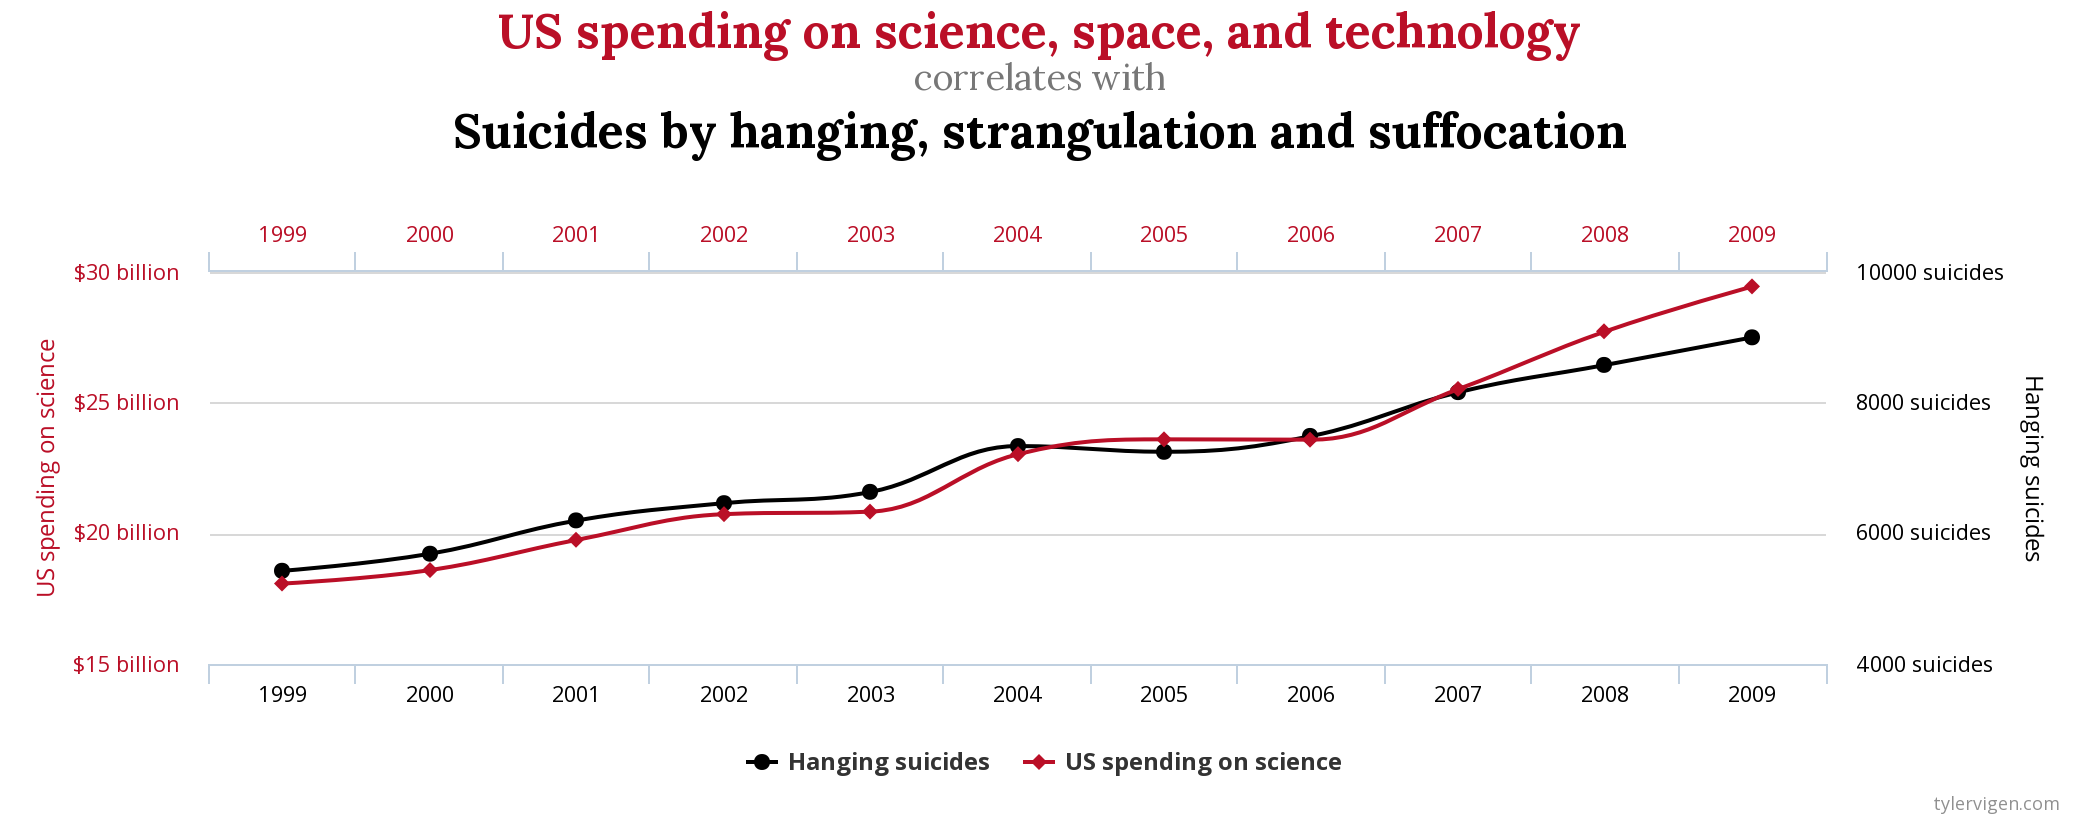
\includegraphics{chart.png}
\caption{}
\end{figure}

\begin{itemize}
\item
  Although these two factors(Us spending on science, space and
  technology \& Suicides by hanging, strangulation and suffocation) are
  strongly correlated (99.79\%), there's unlikely to have actual
  causality exists between these two factors. Because suicide rate and
  science and technology funding are basically two distinct fields, the
  occurrence of neither one could be applied to explain why the other's
  changes. The increase of Us spending on science does not contribute to
  the ascending trend of hanging suicide rate, and vice versa.
\item
  \textbf{The US annual GDP growth} has a causative link with \textbf{US
  spending on science and technology}. With a more promising economic
  growth, the funding poured into the field of science research will be
  more likely to increase. And with significant amount of spending on
  technological research, the revolutionary outcomes could contribute
  back to the country's economic development, therefore creating a
  virtuous circle.
\end{itemize}

    \subsubsection*{Q5}\label{q5}

    5.Let \(X \sim N(2, 6)\) and \(Y \sim N(-3, 2)\) and \(Z \sim N(0, 1)\).
All three random variables are independent of each other. Do the
following. Show all work.

\begin{itemize}
\item
  \begin{enumerate}
  \def\labelenumi{(\alph{enumi})}
  \tightlist
  \item
    What is the distribution of W = X + Y + Z ? What are E(W) and
    Var(W)?
  \end{enumerate}
\item
  \begin{enumerate}
  \def\labelenumi{(\alph{enumi})}
  \setcounter{enumi}{1}
  \tightlist
  \item
    What is the distribution of Q = 2Y ?
  \end{enumerate}
\item
  \begin{enumerate}
  \def\labelenumi{(\alph{enumi})}
  \setcounter{enumi}{2}
  \tightlist
  \item
    What is the distribution of P = -2X + 4?
  \end{enumerate}
\item
  \begin{enumerate}
  \def\labelenumi{(\alph{enumi})}
  \setcounter{enumi}{3}
  \tightlist
  \item
    Find a and b so that M = a + bX is distributed as a standard Normal
    distribution.
  \end{enumerate}
\end{itemize}

    \begin{itemize}
\item
  \begin{enumerate}
  \def\labelenumi{(\alph{enumi})}
  \tightlist
  \item
    Since \(X \sim N(2, 6), Y \sim N(-3, 2), Z \sim N(0, 1)\),
  \end{enumerate}
\end{itemize}

and the rule of variance:

\[Var(x+y) = Var(x) + Var(y) + 2cov(x,y)\]

according to what's denoted in the question, all three random variables
are independent of each other,

\[\therefore Var(x+y) = Var(x) + Var(y)\]

\[\therefore W \sim N(2-3+0, 6+2+1) = N(-1, 9)\]

\[\therefore E(W) = -1, Var(W) = 9\]

    \begin{itemize}
\item
  \begin{enumerate}
  \def\labelenumi{(\alph{enumi})}
  \setcounter{enumi}{1}
  \tightlist
  \item
    Since \(Y \sim N(-3, 2)\),
  \end{enumerate}
\end{itemize}

and the rule of mean:

\[E(cX) = cE(X)\]

the rule of variance:

\[Var(cX) = c^2 Var(X)\]

\[\therefore Q \sim N(2 \cdot (-3), 2^2 \cdot 2)\]

\[Q \sim N(-6, 8)\]

    \begin{itemize}
\item
  \begin{enumerate}
  \def\labelenumi{(\alph{enumi})}
  \setcounter{enumi}{2}
  \tightlist
  \item
    according to the rules discussed in part (b), we know that:
  \end{enumerate}
\end{itemize}

\[E(cX) = cE(X)\]

\[Var(cX) = c^2 Var(X)\]

\[\therefore (-2X) \sim N((-2) \cdot 2, (-2)^2 \cdot 6)\]

\[\therefore (-2X) \sim N(-4, 24)\]

and the rule of mean:

\[E(X+c) = E(X) +c\]

the rule of variance:

\[Var(X+c) = E[(X+c)^2] - [E(X+c)]^2 = E(X^2) - [E(X)]^2 = Var(X)\]

\[\therefore P = -2X + 4 \sim N(-4+4, 24)\]

\[\therefore P = -2X + 4 \sim N(0, 24)\]

    \begin{itemize}
\item
  \begin{enumerate}
  \def\labelenumi{(\alph{enumi})}
  \setcounter{enumi}{3}
  \tightlist
  \item
    according the rules of mean and variance discussed in all parts
    above
  \end{enumerate}
\end{itemize}

\[M = a+bX \sim N(2b+a, 6b^2)\]

if \(M\)is distributed as a standard Normal distribution, then \(M\) is
a normal distribution with a mean of 0 and a standard deviation of 1

\begin{align}
\left\{\begin{matrix} 2b+a=0
\\ 6b^2 = 1
\end{matrix}\right.\end{align}

therefore:

\begin{align}
\left\{\begin{matrix} a = - \frac{\sqrt{6}}{3}
\\ b = \frac{\sqrt{6}}{6}
\end{matrix}\right.\end{align}

or

\begin{align}
\left\{\begin{matrix} a = \frac{\sqrt{6}}{3}
\\ b = -\frac{\sqrt{6}}{6}
\end{matrix}\right.\end{align}

    \subsubsection*{Q6}\label{q6}

    6.Do the following

\begin{itemize}
\item
  \begin{enumerate}
  \def\labelenumi{(\alph{enumi})}
  \tightlist
  \item
    Use R to simulate 1000 iid random variables \({X_i}\) with
    \(Xi \sim N(-2, 3)\). Plot a histogram of your simulated values.
  \end{enumerate}
\item
  \begin{enumerate}
  \def\labelenumi{(\alph{enumi})}
  \setcounter{enumi}{1}
  \tightlist
  \item
    Also simulate 1000 iid random variables \({Y_i}\) with
    \(Y_i \sim (3, 1)\). Plot a histogram of your simulated values.
  \end{enumerate}
\item
  \begin{enumerate}
  \def\labelenumi{(\alph{enumi})}
  \setcounter{enumi}{2}
  \tightlist
  \item
    Finally, plot a histogram of \({Zi}\), where \(Z_i = X_i + Y_i\).
  \end{enumerate}
\item
  \begin{enumerate}
  \def\labelenumi{(\alph{enumi})}
  \setcounter{enumi}{3}
  \tightlist
  \item
    Is \(Z_i\) independent of \(X_i\)? Explain your answer.
  \end{enumerate}
\item
  \begin{enumerate}
  \def\labelenumi{(\alph{enumi})}
  \setcounter{enumi}{4}
  \tightlist
  \item
    Find the sample mean and variance of the Zis you simulated, and
    compare them with the true, theoretical mean and variance.
  \end{enumerate}
\end{itemize}

    \begin{itemize}
\item
  \begin{enumerate}
  \def\labelenumi{(\alph{enumi})}
  \item
  \end{enumerate}
\end{itemize}

    \begin{Verbatim}[commandchars=\\\{\}]
{\color{incolor}In [{\color{incolor}122}]:} X\PY{o}{=}rnorm\PY{p}{(}\PY{l+m}{1000}\PY{p}{,}mean\PY{o}{=}\PY{l+m}{\PYZhy{}2}\PY{p}{,}sd\PY{o}{=}\PY{k+kp}{sqrt}\PY{p}{(}\PY{l+m}{3}\PY{p}{)}\PY{p}{)}
\end{Verbatim}


    \begin{Verbatim}[commandchars=\\\{\}]
{\color{incolor}In [{\color{incolor}142}]:} \PY{k+kn}{library}\PY{p}{(}ggplot2\PY{p}{)}
          X\PYZus{}df \PY{o}{=} \PY{k+kt}{data.frame}\PY{p}{(}x \PY{o}{=} X\PY{p}{)}
          ggplot\PY{p}{(}X\PYZus{}df\PY{p}{,} aes\PY{p}{(}x \PY{o}{=} x\PY{p}{)}\PY{p}{)} \PY{o}{+} 
              geom\PYZus{}histogram\PY{p}{(}aes\PY{p}{(}y \PY{o}{=}\PY{l+m}{.}\PY{l+m}{.}density..\PY{p}{)}\PY{p}{)} \PY{o}{+}
              ggtitle\PY{p}{(}\PY{l+s}{\PYZdq{}}\PY{l+s}{Histogram of X∼N(−2,3)\PYZdq{}}\PY{p}{)}\PY{o}{+}
              theme\PY{p}{(}plot.title \PY{o}{=} element\PYZus{}text\PY{p}{(}hjust \PY{o}{=} \PY{l+m}{0.5}\PY{p}{)}\PY{p}{)} \PY{o}{+}
              stat\PYZus{}function\PY{p}{(}fun \PY{o}{=} dnorm\PY{p}{,} args \PY{o}{=} \PY{k+kt}{list}\PY{p}{(}mean \PY{o}{=} \PY{l+m}{\PYZhy{}2}\PY{p}{,} 
                                                     sd \PY{o}{=} \PY{k+kp}{sqrt}\PY{p}{(}\PY{l+m}{3}\PY{p}{)}\PY{p}{)}\PY{p}{,} col\PY{o}{=}\PY{l+s}{\PYZsq{}}\PY{l+s}{blue\PYZsq{}}\PY{p}{,} lwd\PY{o}{=}\PY{l+m}{1}\PY{p}{)}
\end{Verbatim}


    \begin{Verbatim}[commandchars=\\\{\}]
`stat\_bin()` using `bins = 30`. Pick better value with `binwidth`.

    \end{Verbatim}

    
    
    \begin{center}
    \adjustimage{max size={0.7\linewidth}{0.7\paperheight}}{output_23_2.png}
    \end{center}
    { \hspace*{\fill} \\}
    
    \begin{itemize}
\item
  \begin{enumerate}
  \def\labelenumi{(\alph{enumi})}
  \setcounter{enumi}{1}
  \item
  \end{enumerate}
\end{itemize}

    \begin{Verbatim}[commandchars=\\\{\}]
{\color{incolor}In [{\color{incolor}143}]:} Y \PY{o}{=} rnorm\PY{p}{(}\PY{l+m}{1000}\PY{p}{,}mean\PY{o}{=}\PY{l+m}{3}\PY{p}{,}sd\PY{o}{=}\PY{k+kp}{sqrt}\PY{p}{(}\PY{l+m}{1}\PY{p}{)}\PY{p}{)}
\end{Verbatim}


    \begin{Verbatim}[commandchars=\\\{\}]
{\color{incolor}In [{\color{incolor}144}]:} Y\PYZus{}df \PY{o}{=} \PY{k+kt}{data.frame}\PY{p}{(}y \PY{o}{=} Y\PY{p}{)}
          ggplot\PY{p}{(}Y\PYZus{}df\PY{p}{,} aes\PY{p}{(}x \PY{o}{=} y\PY{p}{)}\PY{p}{)} \PY{o}{+} 
              geom\PYZus{}histogram\PY{p}{(}aes\PY{p}{(}y \PY{o}{=}\PY{l+m}{.}\PY{l+m}{.}density..\PY{p}{)}\PY{p}{)} \PY{o}{+}
              ggtitle\PY{p}{(}\PY{l+s}{\PYZdq{}}\PY{l+s}{Histogram of Y∼N(3,1)\PYZdq{}}\PY{p}{)}\PY{o}{+}
              theme\PY{p}{(}plot.title \PY{o}{=} element\PYZus{}text\PY{p}{(}hjust \PY{o}{=} \PY{l+m}{0.5}\PY{p}{)}\PY{p}{)} \PY{o}{+}
              stat\PYZus{}function\PY{p}{(}fun \PY{o}{=} dnorm\PY{p}{,} args \PY{o}{=} \PY{k+kt}{list}\PY{p}{(}mean \PY{o}{=} \PY{l+m}{3}\PY{p}{,} 
                                                     sd \PY{o}{=} \PY{k+kp}{sqrt}\PY{p}{(}\PY{l+m}{1}\PY{p}{)}\PY{p}{)}\PY{p}{,} col\PY{o}{=}\PY{l+s}{\PYZsq{}}\PY{l+s}{blue\PYZsq{}}\PY{p}{,} lwd\PY{o}{=}\PY{l+m}{1}\PY{p}{)}
\end{Verbatim}


    \begin{Verbatim}[commandchars=\\\{\}]
`stat\_bin()` using `bins = 30`. Pick better value with `binwidth`.

    \end{Verbatim}

    
    
    \begin{center}
    \adjustimage{max size={0.7\linewidth}{0.7\paperheight}}{output_26_2.png}
    \end{center}
    { \hspace*{\fill} \\}
    
    \begin{itemize}
\item
  \begin{enumerate}
  \def\labelenumi{(\alph{enumi})}
  \setcounter{enumi}{2}
  \item
  \end{enumerate}
\end{itemize}

Since \(Z = X+Y \sim N(-2+3, 3+1)\), thus \(Z \sim N(1, 4)\)

    \begin{Verbatim}[commandchars=\\\{\}]
{\color{incolor}In [{\color{incolor}145}]:} Z \PY{o}{=} rnorm\PY{p}{(}\PY{l+m}{1000}\PY{p}{,}mean\PY{o}{=}\PY{l+m}{1}\PY{p}{,}sd\PY{o}{=}\PY{k+kp}{sqrt}\PY{p}{(}\PY{l+m}{4}\PY{p}{)}\PY{p}{)}
\end{Verbatim}


    \begin{Verbatim}[commandchars=\\\{\}]
{\color{incolor}In [{\color{incolor}146}]:} Z\PYZus{}df \PY{o}{=} \PY{k+kt}{data.frame}\PY{p}{(}z \PY{o}{=} Z\PY{p}{)}
          ggplot\PY{p}{(}Z\PYZus{}df\PY{p}{,} aes\PY{p}{(}x \PY{o}{=} z\PY{p}{)}\PY{p}{)} \PY{o}{+} 
              geom\PYZus{}histogram\PY{p}{(}aes\PY{p}{(}y \PY{o}{=}\PY{l+m}{.}\PY{l+m}{.}density..\PY{p}{)}\PY{p}{)} \PY{o}{+}
              ggtitle\PY{p}{(}\PY{l+s}{\PYZdq{}}\PY{l+s}{Histogram of Z∼N(1,4)\PYZdq{}}\PY{p}{)}\PY{o}{+}
              theme\PY{p}{(}plot.title \PY{o}{=} element\PYZus{}text\PY{p}{(}hjust \PY{o}{=} \PY{l+m}{0.5}\PY{p}{)}\PY{p}{)} \PY{o}{+}
              stat\PYZus{}function\PY{p}{(}fun \PY{o}{=} dnorm\PY{p}{,} args \PY{o}{=} \PY{k+kt}{list}\PY{p}{(}mean \PY{o}{=} \PY{l+m}{1}\PY{p}{,} 
                                                     sd \PY{o}{=} \PY{k+kp}{sqrt}\PY{p}{(}\PY{l+m}{4}\PY{p}{)}\PY{p}{)}\PY{p}{,} col\PY{o}{=}\PY{l+s}{\PYZsq{}}\PY{l+s}{blue\PYZsq{}}\PY{p}{,} lwd\PY{o}{=}\PY{l+m}{1}\PY{p}{)}
\end{Verbatim}


    \begin{Verbatim}[commandchars=\\\{\}]
`stat\_bin()` using `bins = 30`. Pick better value with `binwidth`.

    \end{Verbatim}

    
    
    \begin{center}
    \adjustimage{max size={0.7\linewidth}{0.7\paperheight}}{output_29_2.png}
    \end{center}
    { \hspace*{\fill} \\}
    
    \begin{itemize}
\item
  \begin{enumerate}
  \def\labelenumi{(\alph{enumi})}
  \setcounter{enumi}{3}
  \tightlist
  \item
    Yes, \(Z_i\) is independent of \(X_i\).
  \end{enumerate}
\end{itemize}

Because if two variables are independent of each other, then the
covariance should be close to 0. We already know that \(X\) and \(Y\)
are randomly generated and independent, so:

    \begin{Verbatim}[commandchars=\\\{\}]
{\color{incolor}In [{\color{incolor}147}]:} cov\PY{p}{(}X\PY{p}{,} Y\PY{p}{)}
\end{Verbatim}


    0.0160952090678688

    
    Since \(X\) and \(Y\) are 1000 simulated numbers, we could consider
\(cov(X,Y) \approx 0\)

    \begin{Verbatim}[commandchars=\\\{\}]
{\color{incolor}In [{\color{incolor}148}]:} cov\PY{p}{(}rnorm\PY{p}{(}\PY{l+m}{10000}\PY{p}{,}mean\PY{o}{=}\PY{l+m}{\PYZhy{}2}\PY{p}{,}sd\PY{o}{=}\PY{k+kp}{sqrt}\PY{p}{(}\PY{l+m}{3}\PY{p}{)}\PY{p}{)}\PY{p}{,} rnorm\PY{p}{(}\PY{l+m}{10000}\PY{p}{,}mean\PY{o}{=}\PY{l+m}{3}\PY{p}{,}sd\PY{o}{=}\PY{k+kp}{sqrt}\PY{p}{(}\PY{l+m}{1}\PY{p}{)}\PY{p}{)}\PY{p}{)}
\end{Verbatim}


    0.010238213251291

    
    \begin{Verbatim}[commandchars=\\\{\}]
{\color{incolor}In [{\color{incolor}149}]:} cov\PY{p}{(}rnorm\PY{p}{(}\PY{l+m}{100000}\PY{p}{,}mean\PY{o}{=}\PY{l+m}{\PYZhy{}2}\PY{p}{,}sd\PY{o}{=}\PY{k+kp}{sqrt}\PY{p}{(}\PY{l+m}{3}\PY{p}{)}\PY{p}{)}\PY{p}{,} rnorm\PY{p}{(}\PY{l+m}{100000}\PY{p}{,}mean\PY{o}{=}\PY{l+m}{3}\PY{p}{,}sd\PY{o}{=}\PY{k+kp}{sqrt}\PY{p}{(}\PY{l+m}{1}\PY{p}{)}\PY{p}{)}\PY{p}{)}
\end{Verbatim}


    -0.00922166054983182

    
    \begin{Verbatim}[commandchars=\\\{\}]
{\color{incolor}In [{\color{incolor}150}]:} cov\PY{p}{(}X\PY{p}{,} Z\PY{p}{)}
\end{Verbatim}


    0.0603978617660555

    
    So similarly, \(cov(X, Z) \approx 0\), so it's safe to conclude that
\(Z_i\) is independent of \(X_i\).

    \begin{itemize}
\item
  \begin{enumerate}
  \def\labelenumi{(\alph{enumi})}
  \setcounter{enumi}{4}
  \item
  \end{enumerate}
\end{itemize}

    \begin{Verbatim}[commandchars=\\\{\}]
{\color{incolor}In [{\color{incolor}151}]:} Z\PYZus{}sample\PYZus{}mean \PY{o}{=} \PY{k+kp}{mean}\PY{p}{(}Z\PY{p}{)}
          Z\PYZus{}sample\PYZus{}var \PY{o}{=} var\PY{p}{(}Z\PY{p}{)}
\end{Verbatim}


    \begin{Verbatim}[commandchars=\\\{\}]
{\color{incolor}In [{\color{incolor}152}]:} Z\PYZus{}sample\PYZus{}mean
\end{Verbatim}


    1.00402874538632

    
    \[Z \sim N(1,4)\] \[1.00402874538632 \approx 1\]

    \begin{Verbatim}[commandchars=\\\{\}]
{\color{incolor}In [{\color{incolor}154}]:} Z\PYZus{}sample\PYZus{}var
\end{Verbatim}


    3.74829970236857

    
    \[3.74829970236857 \approx 4\]

    \begin{Verbatim}[commandchars=\\\{\}]
{\color{incolor}In [{\color{incolor}155}]:} ggplot\PY{p}{(}Z\PYZus{}df\PY{p}{,} aes\PY{p}{(}x \PY{o}{=} z\PY{p}{)}\PY{p}{)} \PY{o}{+} 
              geom\PYZus{}histogram\PY{p}{(}aes\PY{p}{(}y \PY{o}{=}\PY{l+m}{.}\PY{l+m}{.}density..\PY{p}{)}\PY{p}{)} \PY{o}{+}
              geom\PYZus{}density\PY{p}{(}alpha\PY{o}{=}\PY{l+m}{0.2}\PY{p}{,} fill\PY{o}{=}\PY{l+s}{\PYZdq{}}\PY{l+s}{\PYZsh{}FF6666\PYZdq{}}\PY{p}{)}\PY{o}{+}
              ggtitle\PY{p}{(}\PY{l+s}{\PYZdq{}}\PY{l+s}{Histogram of X∼N(1,4)\PYZdq{}}\PY{p}{)}\PY{o}{+}
              theme\PY{p}{(}plot.title \PY{o}{=} element\PYZus{}text\PY{p}{(}hjust \PY{o}{=} \PY{l+m}{0.5}\PY{p}{)}\PY{p}{)} \PY{o}{+}
              stat\PYZus{}function\PY{p}{(}fun \PY{o}{=} dnorm\PY{p}{,} args \PY{o}{=} \PY{k+kt}{list}\PY{p}{(}mean \PY{o}{=} \PY{l+m}{1}\PY{p}{,} sd \PY{o}{=} \PY{k+kp}{sqrt}\PY{p}{(}\PY{l+m}{4}\PY{p}{)}\PY{p}{)}\PY{p}{,} 
                            col\PY{o}{=}\PY{l+s}{\PYZsq{}}\PY{l+s}{blue\PYZsq{}}\PY{p}{,} lwd\PY{o}{=}\PY{l+m}{1}\PY{p}{,} type\PY{o}{=}\PY{l+s}{\PYZsq{}}\PY{l+s}{area\PYZsq{}}\PY{p}{)}
\end{Verbatim}


    \begin{Verbatim}[commandchars=\\\{\}]
Warning message:
“Ignoring unknown parameters: type”`stat\_bin()` using `bins = 30`. Pick better value with `binwidth`.

    \end{Verbatim}

    
    
    \begin{center}
    \adjustimage{max size={0.7\linewidth}{0.7\paperheight}}{output_43_2.png}
    \end{center}
    { \hspace*{\fill} \\}
    

    % Add a bibliography block to the postdoc
    
    
    
    \end{document}
